When a load is attached to the main output, there is a voltage drop over the ADP5090 ($V_{\text{BAT}}-V_{\text{SYS}}$ in Figure \ref{development:discharge}). 
This drop causes the chip to switch off the output way too early.
It was necessary to bypass the ADP5090 and connect the receiver circuit directly to the capacitor due to this reason.
This way, the capacitor is not protected from overdischarging, but charging of the capacitor is still controlled by the ADP5090.

Figure \ref{results:v} shows a plot of the voltages of the power supply. 
\begin{figure}[ht]
	\centering
	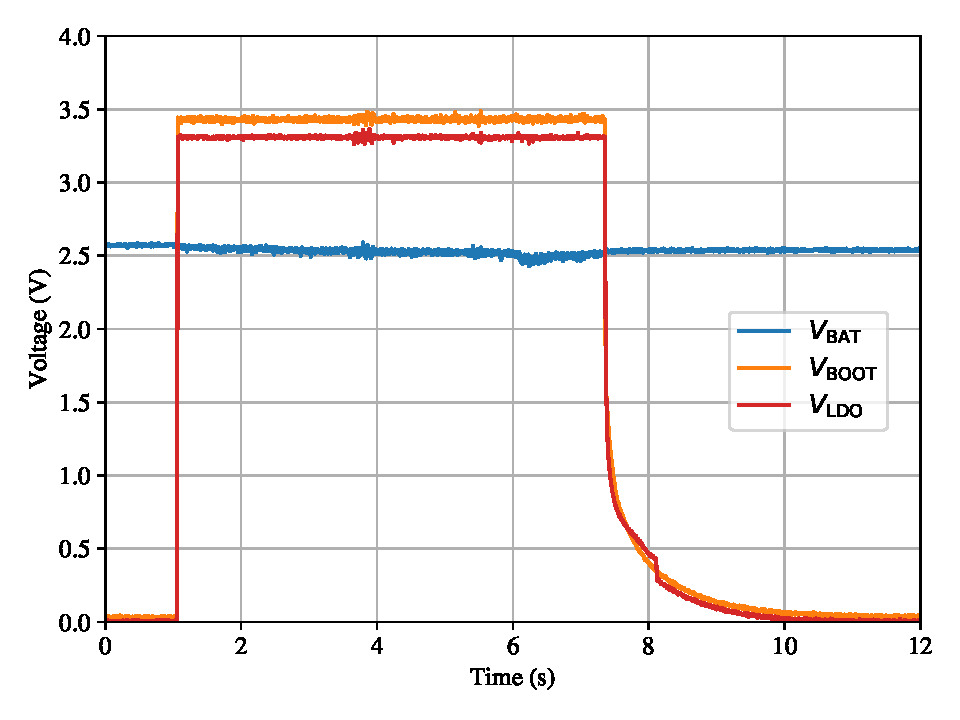
\includegraphics[width=0.9\textwidth]{5-results/power_supply/plot/v.pdf}
	\caption{Power consumption during one write cycle.\label{results:v}}
\end{figure}
The voltage across the capacitor is labelled as $V_{\text{BAT}}$.
Additionally, the voltages after the step-up converter ($V_{\text{BOOT}}$) and LDO ($V_{\text{LDO}}$) were tracked.
The whole power supply manages to provide a stable voltage across the whole write cycle, despite high current peaks.